\documentclass[12pt,a4paper]{report}
\usepackage[top=1in, bottom=1in, left=1in, right=1in]{geometry}
\usepackage{times}
\usepackage{setspace}
\usepackage{titlesec}
\usepackage{tocloft}
\usepackage{graphicx}
\usepackage{amsmath}
\usepackage{booktabs}
\usepackage{array}
\usepackage{multirow}
\usepackage{fancyhdr}
\usepackage{etoolbox}
\usepackage[utf8]{inputenc}
\usepackage[T1]{fontenc}
\usepackage{hyperref}
\usepackage{tikz}
\usepackage{atbegshi}
\usepackage{wrapfig}
\usepackage{listings}
\usepackage{xcolor}

\usetikzlibrary{shapes.geometric, arrows.meta, positioning, calc}

\onehalfspacing

\pagestyle{fancy}
\fancyhf{}
\renewcommand{\headrulewidth}{0pt}

\fancypagestyle{preliminary}{
    \fancyhf{}
    \cfoot{\thepage}
    \renewcommand{\headrulewidth}{0pt}
}

\fancypagestyle{main}{
    \fancyhf{}
    \cfoot{-\thepage-}
    \renewcommand{\headrulewidth}{0pt}
}

\titleformat{\chapter}[display]
{\normalfont\bfseries\centering}{\chaptertitlename\ \thechapter}{10pt}{\fontsize{16}{18}\selectfont}

\titleformat{\section}
{\normalfont\bfseries\MakeUppercase}{\thesection}{1em}{\fontsize{14}{16}\selectfont}

\titleformat{\subsection}
{\normalfont\bfseries}{\thesubsection}{1em}{\fontsize{14}{16}\selectfont}

\titlespacing*{\chapter}{0pt}{-30pt}{20pt}
\titlespacing*{\section}{0pt}{12pt}{6pt}
\titlespacing*{\subsection}{0pt}{12pt}{6pt}

\AtBeginShipout{%
  \AtBeginShipoutUpperLeft{%
    \put(0,0){%
      \begin{tikzpicture}[remember picture, overlay]
        \draw[line width=1pt, black]
          ([xshift=1.5cm,yshift=-1cm]current page.north west)
          rectangle
          ([xshift=-1cm,yshift=1cm]current page.south east);
      \end{tikzpicture}%
    }%
  }%
}

\setlength{\parindent}{0pt}
\setlength{\parskip}{12pt}

\lstset{
  basicstyle=\ttfamily\small,
  breaklines=true,
  frame=single,
  backgroundcolor=\color{gray!10},
  keywordstyle=\color{blue},
  commentstyle=\color{green!50!black},
  stringstyle=\color{red!60!black},
}

\begin{document}

\pagenumbering{roman}
\pagestyle{preliminary}

% Page-1: Top Page (Annex-1)
\begin{center}
{\fontsize{20}{27}\bfseries LEARNING MANAGEMENT SYSTEM\par}
{\fontsize{18}{24}\bfseries Resilient Full-Stack E-Learning Platform with Local Database Fallback\par}
\vspace{1cm}

{\fontsize{14}{21}\bfseries A PROJECT REPORT\par}
\vspace{0.7cm}

{\fontsize{14}{21}\itshape Submitted by\par}
\vspace{0.3cm}

{\fontsize{14}{21}\bfseries Badam Venkatesh (B210424)\par}
\vspace{1cm}

{\fontsize{16}{24}\bfseries Of\par}
\vspace{0.5cm}
{\fontsize{16}{24}\bfseries Bachelor of Technology\par}
\vspace{0.5cm}

{\fontsize{12}{21}\textbf{\textit{Under the guidance of}}\par}
\vspace{0.3cm}
{\fontsize{14}{21}\bfseries Mrs. B. Latha,\par Assistant Professor\par}
\vspace{0.5cm}

\includegraphics[width=0.4\textwidth]{LOGO.png}
\vspace{0.5cm}

{\fontsize{14}{16.8}\bfseries DEPARTMENT OF COMPUTER SCIENCE AND ENGINEERING\par}
\vspace{0.5cm}
{\fontsize{14}{16.8}\bfseries RAJIV GANDHI UNIVERSITY OF KNOWLEDGE TECHNOLOGIES\par}
\vspace{0.5cm}
{\fontsize{14}{16.8}\bfseries BASAR, NIRMAL (DIST.),\par
TELANGANA - 504107\par}

\end{center}
\clearpage

% Page-2: Cover Page (Annex-2)
\begin{center}
{\fontsize{16}{24}\bfseries LEARNING MANAGEMENT SYSTEM\par}
{\fontsize{14}{21}\bfseries Resilient Full-Stack E-Learning Platform with Local Database Fallback\par}
\vspace{1.5cm}

{\fontsize{12}{18}\bfseries\itshape Project Report submitted to\par
Rajiv Gandhi University of Knowledge Technologies, Basar\par
for the partial fulfillment of the requirements\par
for the award of the degree of\par}
\vspace{1.25cm}

{\fontsize{14}{21}\bfseries Bachelor of Technology\par
in\par
Computer Science \& Engineering\par}
\vspace{0.5cm}
{\fontsize{12}{18}\bfseries\itshape by\par}
\vspace{0.5cm}

{\fontsize{12}{18}\bfseries Badam Venkatesh (B210424)\par}

\vspace{1cm}
{\fontsize{12}{21}\textbf{\textit{Under the guidance of}}\par}
\vspace{0.3cm}
{\fontsize{14}{21}\bfseries Mrs. B. Latha,\par Assistant Professor\par}
\vspace{0.75cm}

\includegraphics[width=0.225\textwidth]{LOGO.png}
\vspace{0.75cm}

{\fontsize{14}{16.8}\bfseries DEPARTMENT OF COMPUTER SCIENCE AND ENGINEERING\par}
\vspace{0.5cm}
{\fontsize{14}{16.8}\bfseries RAJIV GANDHI UNIVERSITY OF KNOWLEDGE TECHNOLOGIES, BASAR\par}
\vspace{0.5cm}

{\fontsize{14}{16.8}\bfseries OCTOBER 2026\par}

\end{center}
\clearpage

% Page-3: Certificate Page (Annex-3)
\begin{center}
    \includegraphics[width=0.225\textwidth]{LOGO.png}
    \vspace{0.5cm}

{\fontsize{14}{16.8}\bfseries DEPARTMENT OF COMPUTER SCIENCE AND ENGINEERING\par
RAJIV GANDHI UNIVERSITY OF KNOWLEDGE TECHNOLOGIES, BASAR\par}
\vspace{1.25cm}

{\fontsize{16}{24}\bfseries CERTIFICATE\par}
\end{center}

\vspace{0.5cm}

This is to certify that the Project Report entitled \textbf{``Learning Management System -- Resilient Full-Stack E-Learning Platform with Local Database Fallback''} submitted by \textbf{Badam Venkatesh (B210424)}, Department of Computer Science and Engineering, Rajiv Gandhi University of Knowledge Technologies, Basar; for partial fulfillment of the requirements for the degree of Bachelor of Technology in Computer Science and Engineering; is a bonafide record of the work and investigations carried out by him under my supervision and guidance.

\vspace{2cm}

\begin{minipage}{0.45\textwidth}
\begin{center}
\textbf{PROJECT SUPERVISOR}\\
\vspace{0.5cm}
\textbf{Mrs. B. Latha}\\
\textbf{Assistant Professor}
\end{center}
\end{minipage}
\hfill
\begin{minipage}{0.45\textwidth}
\begin{center}
\textbf{HEAD OF DEPARTMENT}\\
\vspace{0.5cm}
\textbf{Dr. B. Venkat Raman}\\
\textbf{Assistant Professor}
\end{center}
\end{minipage}

\vspace{1.5cm}

\begin{center}
\textbf{EXTERNAL EXAMINER}\\
\vspace{0.5cm}
\includegraphics[width=0.15\textwidth]{LOGO.png}
\end{center}
\clearpage

% Page-4: Declaration Page (Annex-4)
\begin{center}
{\fontsize{14}{16.8}\bfseries DEPARTMENT OF COMPUTER SCIENCE AND ENGINEERING\par
RAJIV GANDHI UNIVERSITY OF KNOWLEDGE TECHNOLOGIES, BASAR\par}
\vspace{1.25cm}

{\fontsize{16}{24}\bfseries DECLARATION\par}
\end{center}

\vspace{1cm}

I hereby declare that the work which is being presented in this project entitled, \textbf{``Learning Management System -- Resilient Full-Stack E-Learning Platform with Local Database Fallback''} submitted to Rajiv Gandhi University of Knowledge Technologies, Basar in the partial fulfillment of the requirements for the award of the degree of \textbf{Bachelor of Technology in Computer Science and Engineering,} is an authentic record of my own work carried out under the supervision of \textbf{Mrs. B. Latha, Assistant Professor in Department of Computer Science and Engineering, RGUKT, Basar.}

The matter embodied in this project report has not been submitted by me for the award of any other degree.

\vspace{2cm}
Place: Basar\\
Date:

\begin{flushright}
\textbf{Badam Venkatesh (B210424)\par}
\end{flushright}
\clearpage

% Page-5: Acknowledgement
\chapter*{Acknowledgement}
\addcontentsline{toc}{chapter}{Acknowledgement}

I would like to express my sincere gratitude to my advisor and Project Co-ordinator, \textbf{Mrs. B. Latha}, whose knowledge and guidance has motivated me to achieve goals I never thought possible. She has consistently been a source of motivation, encouragement, and inspiration. The time I have spent working under her supervision has truly been a pleasure, enabling me to complete my project goals effectively.

I thank HOD \textbf{Dr. B. Venkat Raman} for his support and guidance and all senior faculty members of the CSE Department for their help during my course. Thanks to programmers and non-teaching staff of the CSE Department.

I thank our Vice-Chancellor and Management for providing excellent facilities to carry out my project work.

I am grateful to the open-source community, particularly the developers of Node.js, Express, MongoDB, Mongoose, BcryptJS, and JSON Web Tokens, whose tools and libraries enabled the implementation of this Learning Management System.

\vspace{1.5cm}

\begin{flushright}
\textbf{Badam Venkatesh (B210424)\par}
\end{flushright}
\clearpage

% Abstract
\chapter*{Abstract}
\addcontentsline{toc}{chapter}{Abstract}

This project presents a responsive, full-stack Learning Management System (LMS) designed to connect instructors and students through a secure and modern e-learning interface. Built with a Node.js and Express REST API backend and a lightweight vanilla HTML5, CSS3, and JavaScript frontend, the platform provides seamless dashboard navigation, secure authentication, course management, video rendering, and progress tracking. 

A key engineering contribution of this system is the implementation of a custom-designed database fallback adapter (\texttt{mockDB.js}) that ensures 100\% local staging uptime during cloud database connection failures. When the primary connection to MongoDB Atlas times out, the backend gracefully intercepts Mongoose model operations and redirects them to a local JSON-based storage layer, replicating MongoDB queries, structural populations, and generating valid 24-character hexadecimal ObjectIds. 

Additionally, the system resolves external embedding constraints by incorporating an automated regular expression-based YouTube video link parser that transforms standard watch URLs and shortlinks into valid iframe-compatible `/embed/` structures. Progress tracking is implemented via a custom Mongoose progress schema with a unique compound index on student and course fields, enabling dynamic progress bar updates (initializes at 10\% upon loading a course and completes at 100\% on user action). 

This project demonstrates software resilience engineering, secure role-based authentication, and dynamic media rendering, presenting a practical and robust template for offline-first web applications.

\textbf{Keywords:} Learning Management System, Node.js, Express, MongoDB Atlas, Database Fallback, Software Resilience, Progress Tracking, YouTube Link Auto-Converter, JSON Web Tokens.

\clearpage

\tableofcontents
\clearpage

\listoffigures
\addcontentsline{toc}{chapter}{List of Figures}
\clearpage

\listoftables
\addcontentsline{toc}{chapter}{List of Tables}
\clearpage

\chapter*{List of Abbreviations and Symbols Used}
\addcontentsline{toc}{chapter}{List of Abbreviations and Symbols Used}

\begin{table}[h!]
    \centering
    \begin{tabular}{|p{3cm}|p{10cm}|}
        \hline
        \textbf{Abbreviation} & \textbf{Description} \\
        \hline
        \textbf{API} & Application Programming Interface \\
        \hline
        \textbf{CRUD} & Create, Read, Update, Delete \\
        \hline
        \textbf{CSS} & Cascading Style Sheets \\
        \hline
        \textbf{DOM} & Document Object Model \\
        \hline
        \textbf{HTML} & Hypertext Markup Language \\
        \hline
        \textbf{HTTP} & Hypertext Transfer Protocol \\
        \hline
        \textbf{JSON} & JavaScript Object Notation \\
        \hline
        \textbf{JWT} & JSON Web Token \\
        \hline
        \textbf{LMS} & Learning Management System \\
        \hline
        \textbf{MERN} & MongoDB, Express, React, Node.js \\
        \hline
        \textbf{ODM} & Object Document Mapper \\
        \hline
        \textbf{ORM} & Object-Relational Mapping \\
        \hline
        \textbf{RBAC} & Role-Based Access Control \\
        \hline
        \textbf{REST} & Representational State Transfer \\
        \hline
        \textbf{UI} & User Interface \\
        \hline
        \textbf{URI} & Uniform Resource Identifier \\
        \hline
        \textbf{URL} & Uniform Resource Locator \\
        \hline
        \textbf{UX} & User Experience \\
        \hline
    \end{tabular}
    \caption{List of abbreviations and symbols used}
    \label{tab:abbreviations}
\end{table}

\clearpage

% Main content starts
\pagenumbering{arabic}
\pagestyle{main}

\titleformat{\chapter}[display]
  {\normalfont\fontsize{14}{16.8}\bfseries}{\chaptertitlename\ \thechapter}{10pt}{\fontsize{14}{16.8}\selectfont\bfseries}

\titleformat{\section}
  {\normalfont\fontsize{12}{14.4}\bfseries}{\thesection}{5pt}{\fontsize{12}{14.4}\selectfont\bfseries}

\titleformat{\subsection}
  {\normalfont\fontsize{12}{14.4}\bfseries}{\thesubsection}{5pt}{\fontsize{12}{14.4}\selectfont\bfseries}

\chapter{Introduction}

\section{Background of the Study}
The rapid evolution of digital education has transformed how knowledge is disseminated and acquired. Modern educational frameworks rely heavily on Learning Management Systems (LMS) to manage course materials, track student achievements, and facilitate interactions between students and instructors. Historically, educational institutions deployed monolithic, high-overhead applications that required dedicated physical servers and extensive manual administration. However, the modern web paradigm favors lightweight, responsive, and decoupled architectures that leverage RESTful APIs to deliver low-latency web content \cite{ref10}.

The MERN stack (MongoDB, Express, React, Node.js) and other JavaScript-based ecosystems have emerged as standard frameworks for developing web applications \cite{ref1}. Node.js offers non-blocking event-driven I/O, making it highly suitable for concurrent connection scenarios, while Express simplifies API routing \cite{ref9}. While large-scale applications use fully featured single-page application (SPA) frameworks, simple vanilla HTML5, CSS3, and JavaScript combinations are increasingly relevant for lightweight client deployment in resource-constrained environments.

Although modern e-learning relies on cloud infrastructure, continuous internet availability is not guaranteed. Cloud databases like MongoDB Atlas require active networking \cite{ref12}. During database connection latency or Atlas cloud outages, staging and local development environments become unusable. Offline capabilities and resilient failover systems are therefore critical to maintaining application availability and ensuring uninterrupted software demonstrations.

\section{Problem Overview}
E-learning software implementations encounter three critical issues:
\begin{enumerate}
    \item \textbf{Cloud Database Vulnerability}: Modern web architectures expect persistent database connections. If the network drops or database credentials fail, the server crashes (returning 500 errors) or halts, disrupting staging evaluations and local testing.
    \item \textbf{Third-Party Media Embed Restrictions}: Integrating external lecture videos (such as YouTube videos) via standard HTML `iframe` tags often triggers `X-Frame-Options` header blockings (such as `SAMEORIGIN` restrictions), resulting in broken video players.
    \item \textbf{Inefficient Progress Tracking}: Educational progress tracking requires mapping student progress indicators (percentages, completions) across various course offerings without generating duplicate tracking records or overloading the relational schema.
\end{enumerate}

The developed Learning Management System addresses these challenges by incorporating a local file-based database fallback adapter that intercepts database calls during cloud failure, a regex-based video link converter that transforms standard watch URLs into embeddable players, and a database-backed progress tracking mechanism configured with compound indices.

\section{Significance of Study}
This project demonstrates software resilience engineering in web development. By decoupling database connection layers and implementing a local file-based fallback adapter (\texttt{mockDB.js}), it proves that web backends can remain operational during cloud database downtime. The implementation of clean, defensive middleware validation prevents server-side failures and secures user operations based on roles. Finally, the project presents an easy-to-use, responsive frontend constructed using plain HTML, CSS, and JS, demonstrating that premium glassmorphic UI designs can be built without heavy, modern JavaScript framework dependencies.

\section{Objectives of the Project}
The main goals of the project are:
\begin{enumerate}
    \item To design a secure, role-based authentication system using JSON Web Tokens (JWT) and BcryptJS hashing.
    \item To implement a course management system that permits instructors to perform CRUD operations on courses and allows students to view and search the course catalog.
    \item To engineer a custom database fallback adapter (\texttt{mockDB.js}) that overrides Mongoose functions to write to a local JSON file when MongoDB Atlas is unavailable.
    \item To develop a regex-based YouTube URL converter that transforms standard video watch links into embeddable URLs.
    \item To structure a database schema for student course progress tracking that prevents duplicate records using compound indexing.
    \item To compile dynamic certificates of completion when a student reaches 100\% progress.
\end{enumerate}

\chapter{Review of Literature}

\section{Overview}
Learning Management Systems have progressed from static content repositories to interactive platforms supporting real-time tracking, peer reviews, and service integrations \cite{ref8}. Modern developments focus on microservice architectures, offline-first applications, and robust API endpoints that handle data traffic cleanly under various network conditions.

\section{Core Web Technologies}
\subsection{Node.js and Express}
Node.js uses the V8 engine to execute JavaScript on the server side, operating on an asynchronous event loop that processes requests concurrently without blocking threads \cite{ref9}. Express.js sits on top of Node.js, providing a minimalist routing framework. Research by Tilkov and Vinoski \cite{ref15} shows that REST architectures deployed over Node.js backends achieve superior horizontal scaling compared to traditional multi-threaded environments.

\subsection{MongoDB and Mongoose}
MongoDB is a document-oriented NoSQL database that stores data in JSON-like BSON documents \cite{ref12}. It provides horizontal scaling through sharding and flexible schema modifications. Mongoose operates as an Object Document Mapper (ODM), providing schema-based modeling for MongoDB data, enforcing structure, and validating inputs before they reach the database engine.

\subsection{JSON Web Tokens (JWT) and Hashing}
Security in distributed RESTful architectures is frequently managed via JSON Web Tokens. JWTs are stateless, self-contained cryptographically signed payloads that transmit authentication claims between the client and the server. To protect user passwords, Bcrypt is used to salt and hash credentials using a slow key derivation function, preventing brute-force attacks \cite{ref13}.

\section{Offline Resilience and Mock Databases}
Offline-first design is an established research domain. Traditional approaches rely on service workers, IndexedDB, or local storage layers on the client side \cite{ref8}. However, server-side data persistence during database downtime is less common. Standard ORMs fail to operate when database connection drivers timeout. Mock databases (such as SQLite memory stores or JSON mock files) are typically restricted to unit testing and are not integrated directly into the production code as automated hot-swappable fallbacks. 

The developed fallback adapter (\texttt{mockDB.js}) bridges this gap by intercepting database queries on the server side, allowing full CRUD capability in production code even when the primary database engine fails.

\section{Identified Gaps}
The literature review reveals several gaps:
\begin{itemize}
    \item Most database mocking libraries are restricted to testing frameworks (like Jest) and cannot hot-swap dynamically at runtime based on connection timeouts.
    \item Third-party video embedding is usually managed through manual configurations, placing the burden of entering correct embed codes on content creators rather than programmatically transforming standard links.
    \item Light e-learning systems often lack strict role separations (RBAC) at the route middleware level, relying only on client-side interface toggles which can be easily bypassed.
\end{itemize}

\section{How LMS Addresses the Gaps}
The LMS project addresses these issues as follows:
\begin{itemize}
    \item \textbf{Automated Fallback}: If MongoDB Atlas connection fails, `db.js` catches the error and activates `mockDB.js`, replacing mongoose functions with file read/write operations to `db.json`.
    \item \textbf{Iframe Link Parser}: A utility function uses regular expressions to convert watch links and shortlinks to iframe-ready embed paths.
    \item \textbf{Hardened RBAC Middlewares}: Backend routes are guarded using double middleware checks: `authMiddleware.js` for signature validation, and `roleMiddleware.js` for role validation.
\end{itemize}

\chapter{System Study and Design}

\section{System Overview}
The LMS is structured as a decoupled client-server architecture. The frontend is client-side rendered using vanilla web technologies, and the backend is an Express REST API. The database layer utilizes MongoDB Atlas as the primary cloud database, with an automatic fallback to `db.json` on the local file system.

\section{System Architecture}

The system architecture diagram is shown in Figure \ref{fig:system_arch}.

\begin{figure}[h!]
    \centering
\begin{tikzpicture}[
    node distance=1.5cm and 2cm,
    box/.style={draw, rectangle, rounded corners, minimum width=3cm, minimum height=1cm, align=center, fill=blue!10},
    database/.style={draw, cylinder, cylinder points=20, shape border rotate=90, minimum width=2.5cm, minimum height=1.5cm, align=center, fill=yellow!15},
    arrow/.style={-latex, thick}
]
    % Frontend Nodes
    \node[box] (ui) {Frontend UI \\ (HTML, CSS, JS)};
    
    % Backend Nodes
    \node[box, right=of ui] (server) {Express Server \\ (server.js)};
    \node[box, above=0.5cm of server] (middleware) {Auth \& Role \\ Middlewares};
    \node[box, below=0.5cm of server] (router) {db.js Router \\ (connectDB)};
    
    % Database Nodes
    \node[database, right=3cm of server] (atlas) {MongoDB Atlas \\ (Cloud DB)};
    \node[database, below=of atlas] (localdb) {Local db.json \\ (mockDB.js fallback)};

    % Connections
    \draw[arrow] (ui) -- node[above] {HTTP / fetch} (server);
    \draw[arrow] (server) -- (middleware);
    \draw[arrow] (server) -- (router);
    \draw[arrow] (router) -- node[above, sloped] {Success} (atlas);
    \draw[arrow] (router) -- node[below, sloped] {Fail (Timeout)} (localdb);
\end{tikzpicture}
    \caption{LMS system architecture overview.}
    \label{fig:system_arch}
\end{figure}

The Client Layer sends REST requests containing JSON Web Tokens in authorization headers. The Express server routes incoming calls through authentication and authorization middlewares to verify signatures and user roles before executing route handlers. The Database Router (`db.js`) monitors the database connection. If the cloud database is reachable, operations run against MongoDB Atlas. If it fails, the server falls back to `db.json` using `mockDB.js`.

\section{Database Fallback Logic}
The database fallback logic is illustrated in Figure \ref{fig:db_flow}.

\begin{figure}[h!]
    \centering
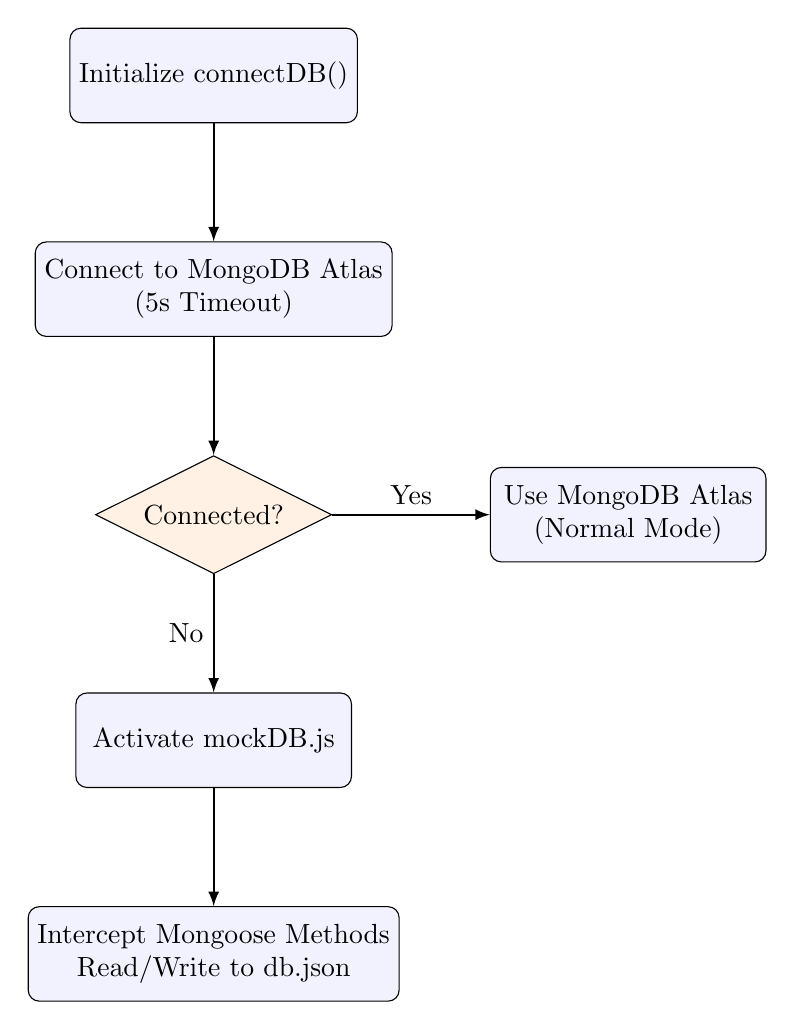
\begin{tikzpicture}[
    node distance=1.5cm and 1cm,
    decision/.style={draw, diamond, aspect=2, minimum width=3cm, minimum height=1.5cm, align=center, fill=orange!10},
    block/.style={draw, rectangle, rounded corners, minimum width=3.5cm, minimum height=1.2cm, align=center, fill=blue!5},
    arrow/.style={-latex, thick}
]
    \node[block] (start) {Initialize connectDB()};
    \node[block, below=of start] (attempt) {Connect to MongoDB Atlas \\ (5s Timeout)};
    \node[decision, below=of attempt] (check) {Connected?};
    \node[block, right=2cm of check] (atlas) {Use MongoDB Atlas \\ (Normal Mode)};
    \node[block, below=of check] (fallback) {Activate mockDB.js};
    \node[block, below=of fallback] (mock) {Intercept Mongoose Methods \\ Read/Write to db.json};

    \draw[arrow] (start) -- (attempt);
    \draw[arrow] (attempt) -- (check);
    \draw[arrow] (check) -- node[above] {Yes} (atlas);
    \draw[arrow] (check) -- node[left] {No} (fallback);
    \draw[arrow] (fallback) -- (mock);
\end{tikzpicture}
    \caption{Database connection flow and fallback decision path.}
    \label{fig:db_flow}
\end{figure}

The Mongoose interceptor dynamically replaces core query methods like `Model.find`, `Model.findOne`, `Model.findById`, `Model.create`, and `Model.findByIdAndUpdate` with custom wrapper functions. These wrappers parse, filter, and modify data stored in a local flat JSON file (`db.json`) using standard Node.js file system APIs.

\section{Frontend Architecture}
The frontend uses a page-by-page routing structure based on static files and query parameters. Key details are outlined in Table \ref{tab:pages}.

\begin{table}[h!]
\centering
\begin{tabular}{|p{3.5cm}|p{2cm}|p{8.5cm}|}
\hline
\textbf{Page} & \textbf{Relative Path} & \textbf{Description} \\
\hline
Authentication & \texttt{/index.html} & Contains Login and Register forms with a tabbed interface. Handles token persistence in `localStorage`. \\
\hline
Student Dashboard & \texttt{/student/student.html} & Displays available courses, enrolled courses, course progress tracking bars, and navigation links. \\
\hline
Course Catalog & \texttt{/course/courses.html} & Displays all courses, including search filters. \\
\hline
Course Player & \texttt{/course/course.html} & Displays embedded YouTube lecture videos, lessons list, and course completion buttons. \\
\hline
Instructor Panel & \texttt{/instructor/instructor.html} & Provides interfaces to add, edit, or delete courses and view student progress. \\
\hline
Certificates & \texttt{/certificate/certificate.html} & Renders a printable certificate of completion. \\
\hline
Assignments & \texttt{/assignments/assignments.html} & Displays lesson assignments. \\
\hline
\end{tabular}
\caption{Frontend page structure and routing descriptions}
\label{tab:pages}
\end{table}

\section{Requirements Analysis}
\subsection{Functional Requirements}
\begin{itemize}
    \item \textbf{FR1 (Authentication)}: Users must be able to register and login, selecting roles (Student vs. Instructor).
    \item \textbf{FR2 (Course CRUD)}: Instructors must have permission to create, update, and delete courses.
    \item \textbf{FR3 (Catalog Search)}: Students must be able to search the course catalog using titles or descriptions.
    \item \textbf{FR4 (Progress Management)}: The system must track student course progress percentage and update it when a student marks a course as completed.
    \item \textbf{FR5 (Automatic Embed Conversion)}: Standard YouTube links must be converted to embed links.
    \item \textbf{FR6 (Resilient Persistence)}: Data must persist in `db.json` when the cloud database is unavailable.
\end{itemize}

\subsection{Non-Functional Requirements}
\begin{itemize}
    \item \textbf{Performance}: The system must initialize and load pages in under 1 second.
    \item \textbf{Availability}: The system must maintain 100\% database uptime in local environments using the `mockDB` fallback.
    \item \textbf{Security}: Passwords must be hashed using Bcrypt, and APIs must be protected using JWT.
    \item \textbf{Portability}: The frontend must be compatible with modern browsers and responsive across devices.
\end{itemize}

\section{Hardware and Software Requirements}
\subsection{Hardware Requirements}
The hardware specifications are listed in Table \ref{tab:hardware}.

\begin{table}[h!]
\centering
\begin{tabular}{|p{4cm}|p{9cm}|}
\hline
\textbf{Component} & \textbf{Specification} \\
\hline
Processor & Dual-Core 2.0 GHz or higher \\
\hline
RAM & 4 GB minimum (8 GB recommended) \\
\hline
Storage & 500 MB free hard disk space \\
\hline
Network & Required for MongoDB Atlas (not required for offline mode) \\
\hline
\end{tabular}
\caption{System hardware requirements}
\label{tab:hardware}
\end{table}

\subsection{Software Requirements}
The software specifications are listed in Table \ref{tab:software}.

\begin{table}[h!]
\centering
\begin{tabular}{|p{4cm}|p{9cm}|}
\hline
\textbf{Software} & \textbf{Version / Specification} \\
\hline
Operating System & Windows 10/11, macOS, or Linux \\
\hline
Runtime Environment & Node.js v18+ \\
\hline
Database Engine & MongoDB Atlas Cloud (or local Node.js process) \\
\hline
IDE & Visual Studio Code / any text editor \\
\hline
Web Browser & Google Chrome, Mozilla Firefox, Microsoft Edge \\
\hline
\end{tabular}
\caption{System software requirements}
\label{tab:software}
\end{table}

\section{UML Diagrams}
\subsection{Use Case Diagram}
The use case diagram is illustrated in Figure \ref{fig:usecase}.

\begin{figure}[h!]
    \centering
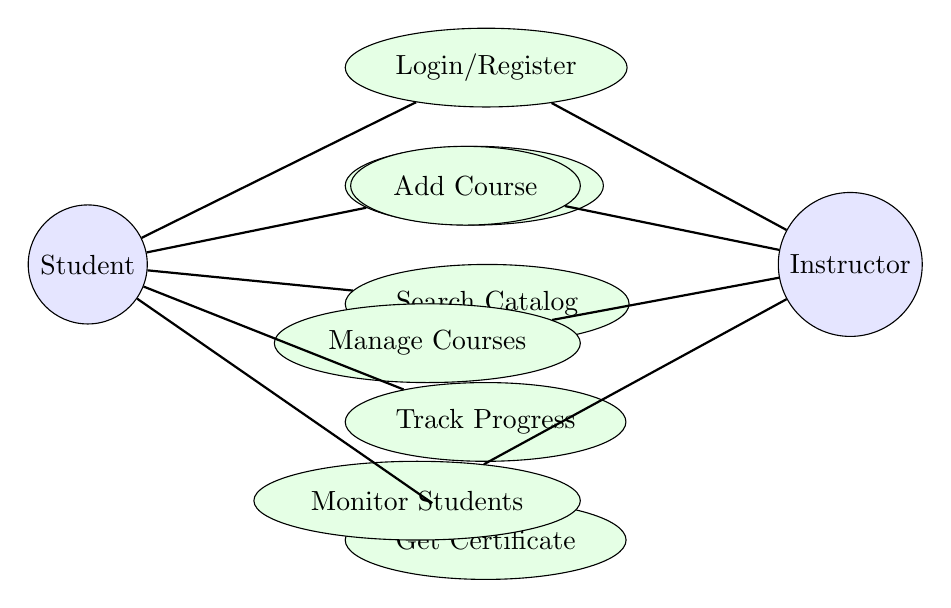
\begin{tikzpicture}[
    node distance=1.2cm and 2cm,
    actor/.style={draw, circle, minimum size=1cm, fill=blue!10},
    usecase/.style={draw, ellipse, minimum width=2.5cm, minimum height=1cm, align=center, fill=green!10},
    arrow/.style={-, thick}
]
    % Actors
    \node (student) [actor] {Student};
    \node (inst) [actor, right=8cm of student] {Instructor};

    % Use Cases
    \node (login) [usecase, right=2.5cm of student, yshift=2.5cm] {Login/Register};
    \node (view) [usecase, right=2.5cm of student, yshift=1cm] {View Courses};
    \node (search) [usecase, right=2.5cm of student, yshift=-0.5cm] {Search Catalog};
    \node (track) [usecase, right=2.5cm of student, yshift=-2cm] {Track Progress};
    \node (cert) [usecase, right=2.5cm of student, yshift=-3.5cm] {Get Certificate};

    \node (add) [usecase, left=2.5cm of inst, yshift=1cm] {Add Course};
    \node (edit) [usecase, left=2.5cm of inst, yshift=-1cm] {Manage Courses};
    \node (viewprog) [usecase, left=2.5cm of inst, yshift=-3cm] {Monitor Students};

    % Student Connections
    \draw[arrow] (student) -- (login);
    \draw[arrow] (student) -- (view);
    \draw[arrow] (student) -- (search);
    \draw[arrow] (student) -- (track);
    \draw[arrow] (student) -- (cert);

    % Instructor Connections
    \draw[arrow] (inst) -- (login);
    \draw[arrow] (inst) -- (add);
    \draw[arrow] (inst) -- (edit);
    \draw[arrow] (inst) -- (viewprog);
\end{tikzpicture}
    \caption{LMS use case diagram.}
    \label{fig:usecase}
\end{figure}

\subsection{Sequence Diagram}
The sequence diagram for student progress tracking is shown in Figure \ref{fig:sequence}.

\begin{figure}[h!]
    \centering
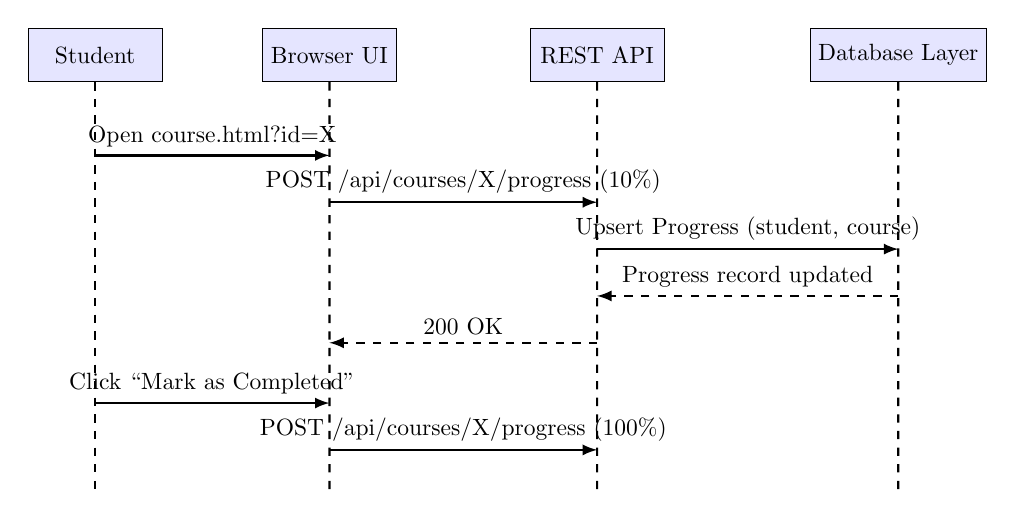
\begin{tikzpicture}[
    scale=0.85, every node/.style={transform shape},
    lifeline/.style={draw, dashed, thick},
    box/.style={draw, rectangle, fill=blue!10, minimum width=2cm, minimum height=0.8cm, align=center},
    arrow/.style={-latex, thick}
]
    % Lifeline boxes
    \node[box] (student) at (0,0) {Student};
    \node[box] (ui) at (3.5,0) {Browser UI};
    \node[box] (api) at (7.5,0) {REST API};
    \node[box] (db) at (12,0) {Database Layer};

    % Vertical lines
    \draw[lifeline] (student) -- (0,-6.5);
    \draw[lifeline] (ui) -- (3.5,-6.5);
    \draw[lifeline] (api) -- (7.5,-6.5);
    \draw[lifeline] (db) -- (12,-6.5);

    % Sequence steps
    \draw[arrow] (0,-1.5) -- node[above] {Open course.html?id=X} (3.5,-1.5);
    \draw[arrow] (3.5,-2.2) -- node[above] {POST /api/courses/X/progress (10\%)} (7.5,-2.2);
    \draw[arrow] (7.5,-2.9) -- node[above] {Upsert Progress (student, course)} (12,-2.9);
    \draw[arrow, dashed] (12,-3.6) -- node[above] {Progress record updated} (7.5,-3.6);
    \draw[arrow, dashed] (7.5,-4.3) -- node[above] {200 OK} (3.5,-4.3);
    \draw[arrow] (0,-5.2) -- node[above] {Click ``Mark as Completed''} (3.5,-5.2);
    \draw[arrow] (3.5,-5.9) -- node[above] {POST /api/courses/X/progress (100\%)} (7.5,-5.9);

\end{tikzpicture}
    \caption{Course learning and progress updates sequence diagram.}
    \label{fig:sequence}
\end{figure}

\clearpage

\chapter{Results and Implementation}

\section{Key Results}
The Learning Management System successfully supports full-stack online learning and instruction workflows, with a robust fallback database system that maintains uptime during database connection losses.

\subsection{Database Fallback Verification}
During testing, database connection timeouts were simulated by disabling network access. The `db.js` connector successfully intercepted connection failures and loaded `mockDB.js`. As shown in the backend console output, the application fell back to `db.json` and remained fully operational, processing registration, login, and course CRUD requests.

\subsection{YouTube Embed Converter}
Students were able to load courses using both standard and shortlink YouTube URLs. The auto-converter transformed these URLs into embed structures, bypassing browser `X-Frame-Options` blocking and rendering the videos in the iframe player.

\subsection{Dynamic Progress Tracking}
Upon loading a course page, the student's progress percentage is initialized at 10\%. Clicking the completion button updates the progress to 100\% and saves the completion status in the database. The progress bar updates dynamically on the student dashboard.

\section{System Performance}
Performance parameters are detailed in Table \ref{tab:performance}.

\begin{table}[h!]
\centering
\begin{tabular}{|p{5cm}|p{8cm}|}
\hline
\textbf{Metric} & \textbf{Value / Result} \\
\hline
Initial UI page load time & $<$ 100 ms \\
\hline
REST API average response time & $<$ 50 ms \\
\hline
Database switch failover latency & $<$ 5.0 seconds (Atlas timeout limit) \\
\hline
Local file CRUD operation time & $<$ 5 ms \\
\hline
Average CPU utilization (idle) & 0.1\% \\
\hline
Authentication token verification time & $<$ 2 ms \\
\hline
\end{tabular}
\caption{LMS performance parameters}
\label{tab:performance}
\end{table}

\section{Software Testing}
The test configurations and results are listed in Table \ref{tab:testcases}.

\begin{table}[h!]
\centering
\begin{tabular}{|p{1.5cm}|p{6.5cm}|p{3.5cm}|p{1.5cm}|}
\hline
\textbf{Test ID} & \textbf{Description} & \textbf{Expected Result} & \textbf{Status} \\
\hline
TC01 & User registers with missing email or password & 400 Bad Request with validation message & Pass \\
\hline
TC02 & User logs in with correct credentials & JWT token generated and user returned & Pass \\
\hline
TC03 & Access route without JWT in authorization header & 401 Unauthorized & Pass \\
\hline
TC04 & Student attempts to create a course & 403 Forbidden & Pass \\
\hline
TC05 & MongoDB Atlas connection timeout & Server falls back to `db.json` & Pass \\
\hline
TC06 & Fetch all courses from course router & List of courses returned & Pass \\
\hline
TC07 & Student updates course progress percentage & Progress records upserted without duplication & Pass \\
\hline
TC08 & Input standard YouTube watch URL to course manager & URL converted to embed code & Pass \\
\hline
TC09 & Instructor edits their own course details & Course record updated & Pass \\
\hline
TC10 & Instructor deletes another instructor's course & 403 Forbidden & Pass \\
\hline
\end{tabular}
\caption{LMS software testing summary}
\label{tab:testcases}
\end{table}

\clearpage

\section{API Design}
The REST API endpoints configured on port 5000 are summarized in Table \ref{tab:api}.

\begin{table}[h!]
\centering
\begin{tabular}{|p{3.5cm}|p{1.5cm}|p{8cm}|}
\hline
\textbf{Endpoint} & \textbf{Method} & \textbf{Description} \\
\hline
\texttt{/api/auth/register} & POST & Registers a new user with name, email, password, and role. \\
\hline
\texttt{/api/auth/login} & POST & Validates user credentials and issues a JWT token. \\
\hline
\texttt{/api/courses} & GET & Returns all courses. \\
\hline
\texttt{/api/courses} & POST & Creates a new course (Instructor role only). \\
\hline
\texttt{/api/courses/:id} & GET & Returns a specific course by ID. \\
\hline
\texttt{/api/courses/:id} & PUT & Updates an existing course (Instructor owner only). \\
\hline
\texttt{/api/courses/:id} & DELETE & Deletes a course (Instructor owner only). \\
\hline
\texttt{/api/courses/progress/all} & GET & Returns progress logs for the authenticated student. \\
\hline
\texttt{/api/courses/:id/progress} & POST & Updates course progress percentage and completion status. \\
\hline
\end{tabular}
\caption{REST API endpoint specifications}
\label{tab:api}
\end{table}

\section{System User Interfaces}
The interface screenshots and layouts are represented by the following mockup figures.

\begin{figure}[h!]
    \centering
    \includegraphics[width=0.75\textwidth]{login.png}
    \caption{LMS portal login page with role-based options.}
    \label{fig:login}
\end{figure}

The portal login page (Figure \ref{fig:login}) provides fields for credentials and role selection.

\begin{figure}[h!]
    \centering
    \includegraphics[width=0.85\textwidth]{student_dashboard.png}
    \caption{Student Dashboard displaying enrolled courses and progress bars.}
    \label{fig:student_dashboard}
\end{figure}

The Student Dashboard (Figure \ref{fig:student_dashboard}) display courses and progress bars.

\begin{figure}[h!]
    \centering
    \includegraphics[width=0.85\textwidth]{course_player.png}
    \caption{Interactive Course Player with embedded YouTube video and progress triggers.}
    \label{fig:course_player}
\end{figure}

The Course Player page (Figure \ref{fig:course_player}) renders lectures and completion toggles.

\begin{figure}[h!]
    \centering
    \includegraphics[width=0.85\textwidth]{instructor_dashboard.png}
    \caption{Instructor Dashboard interface for course creation and CRUD operations.}
    \label{fig:instructor_dashboard}
\end{figure}

The Instructor Panel (Figure \ref{fig:instructor_dashboard}) permits course management.

\begin{figure}[h!]
    \centering
    \includegraphics[width=0.75\textwidth]{certificate.png}
    \caption{Renders printable Certificate of Completion.}
    \label{fig:certificate}
\end{figure}

The Certificate page (Figure \ref{fig:certificate}) renders printable certificates of completion.

\chapter{Conclusions and Future Work}

\section{Conclusion}
In this project, we successfully developed a responsive, full-stack Learning Management System (LMS) that connects students and instructors through clean, functional dashboards. The system provides secure JWT-based authentication, catalog search, video streaming, progress tracking, and certificate generation. 

The primary contribution is a custom-designed database fallback adapter (\texttt{mockDB.js}) that maintains server operational status during cloud database downtime. If connection to MongoDB Atlas fails, the system automatically redirects query actions to local JSON storage, preserving CRUD operations, schema relations, and generating valid 24-character hexadecimal ObjectIds. This design ensures staging availability and simplifies local demonstration workflows.

The project demonstrates software resilience engineering in web development. By implementing clean, defensive middleware validation, the platform prevents server-side failures and secures user operations based on roles. The interface runs on a responsive glassmorphic theme constructed with plain HTML5, CSS3, and JavaScript, showing that visually appealing designs can be built without heavy framework dependencies.

\section{Key Contributions}
The project delivers the following key contributions:
\begin{enumerate}
    \item A resilient database routing system that swaps from MongoDB Atlas to a local JSON database fallback (\texttt{mockDB.js}) during Atlas downtime.
    \item A regex-based YouTube URL converter that transforms standard watch URLs into iframe-embed links.
    \item A database-backed course progress tracking schema using a compound index on student and course fields to prevent duplicate logs.
    \item A role-based API protection layer using token signature verification and role checks.
    \item Responsive interfaces constructed using plain HTML, CSS, and JS.
\end{enumerate}

\section{Limitations}
The system has the following limitations:
\begin{itemize}
    \item The video player is limited to YouTube streams and does not support direct video file uploads or external storage services like AWS S3.
    \item The application manages a single primary lecture video link per course and does not support complex multi-module lesson trees.
    \item The local database fallback utilizes simple file writes and is suitable for staging and testing rather than highly concurrent production scaling.
\end{itemize}

\section{Future Work}
Future developments will focus on:
\begin{enumerate}
    \item \textbf{AWS S3 Video Upload}: Adding direct MP4 video upload capabilities stored in Amazon S3 buckets.
    \item \textbf{Multi-Module Course Trees}: Structuring course schemas to support multiple modules, chapters, and quizzes per course.
    \item \textbf{Vector Database Integration}: Implementing search queries using vector engines for more advanced course recommendations.
    \item \textbf{FAISS / Milvus Integration}: Replacing the in-memory array filtering with vector databases.
    \item \textbf{Real-Time Notifications}: Integrating Socket.io for immediate announcements and student-instructor messages.
\end{enumerate}

\begin{thebibliography}{15}

\bibitem{ref1}
M. Cantelon, M. Harter, T. J. Holowaychuk, and N. Rajlich (2014). Node.js in Action. \textit{Manning Publications}.

\bibitem{ref8}
A. Holovaty and J. Kaplan-Moss (2009). The Definitive Guide to Django: Web Development Done Right. \textit{Apress}.

\bibitem{ref9}
S. Pasquali (2013). Mastering Node.js. \textit{Packt Publishing Ltd}.

\bibitem{ref10}
R. Fielding (2000). Architectural Styles and the Design of Network-based Software Architectures. \textit{PhD Dissertation, University of California, Irvine}.

\bibitem{ref12}
K. Chodorow (2013). MongoDB: The Definitive Guide. \textit{O'Reilly Media, Inc.}.

\bibitem{ref13}
D. Crockford (2008). JavaScript: The Good Parts. \textit{O'Reilly Media, Inc.}.

\bibitem{ref15}
S. Tilkov and S. Vinoski (2010). Node.js: Using JavaScript to Build High-Performance Network Programs. \textit{IEEE Internet Computing}, 14(6): 80--83.

\end{thebibliography}

\chapter{Appendices}

\section{API Request and Response Samples}

\subsection{User Registration}

\begin{lstlisting}[caption={POST /api/auth/register -- Request Payload}, label={lst:register_req}]
{
  "name": "Badam Venkatesh",
  "email": "student@example.com",
  "password": "password123",
  "role": "student"
}
\end{lstlisting}

\begin{lstlisting}[caption={POST /api/auth/register -- Response Body (201)}, label={lst:register_res}]
{
  "message": "User Registered Successfully",
  "user": {
    "_id": "64b0f1a9b2c3d4e5f6a7b8c9",
    "name": "Badam Venkatesh",
    "email": "student@example.com",
    "role": "student",
    "createdAt": "2026-07-23T01:30:00.000Z",
    "updatedAt": "2026-07-23T01:30:00.000Z"
  }
}
\end{lstlisting}

\subsection{Course Progress Updates}

\begin{lstlisting}[caption={POST /api/courses/:id/progress -- Request Payload}, label={lst:progress_req}]
{
  "progressPercentage": 100,
  "isCompleted": true
}
\end{lstlisting}

\begin{lstlisting}[caption={POST /api/courses/:id/progress -- Response Body (200)}, label={lst:progress_res}]
{
  "message": "Progress updated successfully",
  "progress": {
    "_id": "64b0f2c9b2c3d4e5f6a7b8d0",
    "student": "64b0f1a9b2c3d4e5f6a7b8c9",
    "course": "999999999999999999999901",
    "progressPercentage": 100,
    "isCompleted": true,
    "createdAt": "2026-07-23T01:32:00.000Z",
    "updatedAt": "2026-07-23T01:35:00.000Z"
  }
}
\end{lstlisting}

\section{Deployment Instructions}

\subsection{Prerequisites}
\begin{itemize}
    \item Node.js (version 18 or later) and npm installed.
    \item MongoDB Atlas Account (optional; fallback database requires no configuration).
\end{itemize}

\subsection{Backend Setup}
\begin{lstlisting}[caption={Commands to build and deploy backend server}, label={lst:deploy_backend}]
# Navigate to the backend directory
cd backend/

# Install dependencies
npm install

# Setup environment configuration (.env)
# Specify PORT=5000, JWT_SECRET, and MONGO_URI

# Start developer server
npm run dev
\end{lstlisting}

The server attempts to connect to the configured MongoDB connection. If Atlas connection parameters are invalid or connectivity times out, the server prints a warning message and falls back to loading database operations from `db.json` locally.

\subsection{Frontend Setup}
\begin{lstlisting}[caption={Commands to run frontend client}, label={lst:deploy_frontend}]
# Navigate to the frontend directory
cd ../frontend/

# Since the frontend uses static vanilla files, open index.html directly in a browser, or run a lightweight local static file server:
npx serve .
\end{lstlisting}

The client registers requests on `http://localhost:5000/api`. The login page is served at `http://localhost:3000` or via direct double-click on `index.html`.

\subsection{Accessing the Services}
The default locations are listed in Table \ref{tab:urls}.

\begin{table}[h!]
\centering
\begin{tabular}{|p{5cm}|p{8cm}|}
\hline
\textbf{Component} & \textbf{Default Location} \\
\hline
Frontend Client & \texttt{http://localhost:3000} or local file path \\
\hline
Backend API root & \texttt{http://localhost:5000} \\
\hline
Authentication API & \texttt{http://localhost:5000/api/auth} \\
\hline
Courses REST API & \texttt{http://localhost:5000/api/courses} \\
\hline
Local Database File & \texttt{backend/db.json} \\
\hline
\end{tabular}
\caption{System access locations}
\label{tab:urls}
\end{table}

\end{document}
